\chapter{Curriculum Vitae}

\begin{flushright}
  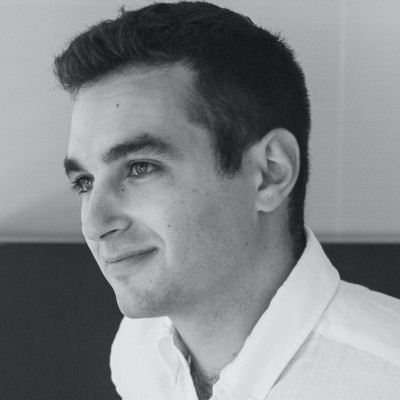
\includegraphics[width=3.2cm]{figures/author.png}
\end{flushright}

\vspace{-1em}

\noindent Joseph Gideon Meyer was born in Toronto, Ontario, Canada. He studied
Electrical Engineering at Tel Aviv University (TAU), receiving his BSc in 2022 and his
MSc in 2024. His master's research, supervised by Prof.\ Ady Arie, addressed
free-space quantum key distribution via spatial modes of light.

\vspace{0.6em}

\noindent Alongside his academic training, from 2021 to 2025 he worked as an
FPGA engineer at Elisra, where he contributed to chip design and algorithm
development and gained hands-on experience with the programmable hardware that
later became central to his doctoral research.

\vspace{0.6em}

\noindent From 2025 to 2026 he pursued a PhD within the QUARC doctoral network,
funded by the Marie Sk\l{}odowska-Curie Actions, as an industrial doctorate at
Eindhoven University of Technology (TU/e) under the supervision of
prof.dr.ir.\ I.~Tafur Monroy and embedded with NVIDIA's networking organization.
His research, carried out at the intersection of integrated photonics,
cryptography, and programmable datacenter hardware, forms the basis of this
dissertation on cross-layer network security in the post-quantum era.

\vspace{0.6em}

\noindent Since 2026 he has been a senior network researcher at NVIDIA, where he
continues to work on quantum-resilient and high-performance networking.
